\subsection{Policy Iteration}
\label{sec:c:pi}

\paragraph{Algorithme en deux phases (Russell \& Norvig, Ch.~17.3 ; Sutton \& Barto, §4.3)}

\textbf{Phase 1 --- \'{E}valuation de politique :}
\begin{equation}
V^{\pi}(s) \leftarrow R\bigl(s,\pi(s)\bigr)
  + \gamma \sum_{s'} P\bigl(s,\pi(s),s'\bigr)\, V^{\pi}(s')
\end{equation}

\textbf{Phase 2 --- Am\'{e}lioration de politique :}
\begin{equation}
\pi_{\text{new}}(s) \leftarrow \arg\max_{a}\left[
  R(s,a) + \gamma \sum_{s'} P(s,a,s')\, V^{\pi}(s') \right]
\end{equation}

\textbf{Param\`{e}tres :} $\gamma = 0.95$, $\varepsilon_{\text{eval}} = 1e-06$, $N = 7$ \'{'}tats, $A = 5$ actions.
Convergence en \textbf{4} it\'{'}ration(s) globale(s)
(1735 it\'{'}rations d'\'{'}valuation cumul\'{'}es, converg\'{e}).

\textit{Note comparative :} PI converge en \textbf{4} it\'{'}ration(s) globale(s) contre \textbf{281} it\'{'}rations Bellman pour VI à $\gamma=0.95$ --- un rapport de 70:1 en faveur de PI (en it\'{'}rations de politique).

\IfFileExists{figures/pi_convergence.png}{%
\begin{figure}[H]
  \centering
  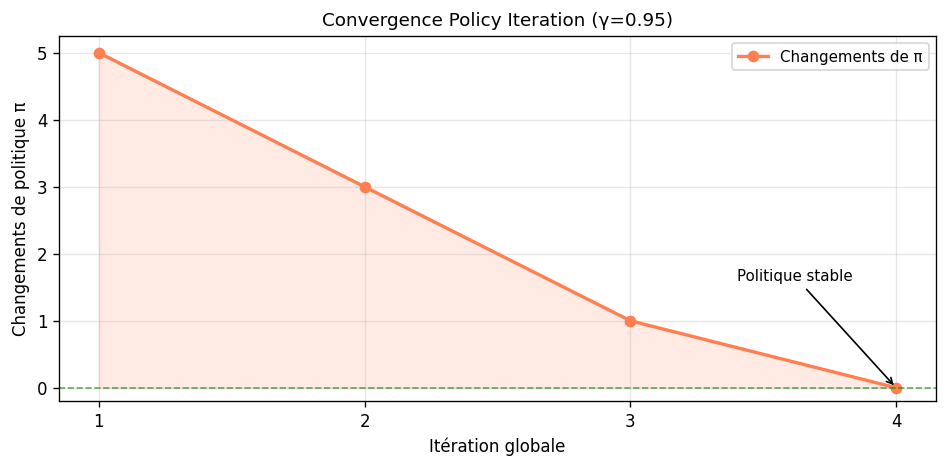
\includegraphics[width=0.85\textwidth]{figures/pi_convergence.png}
  \caption{Convergence Policy Iteration ($\gamma=0.95$) : nombre de changements
    de politique par it\'{e}ration globale. Stabilisation en 4 it\'{e}rations
    (1\,735 it\'{e}rations d'\'{e}valuation cumul\'{e}es).}
  \label{fig:pi_convergence}
\end{figure}}{}

\begin{table}[H]
\centering
\caption{Politique optimale $\pi^*$ --- Policy Iteration ($\gamma=0.95$)}
\label{tab:c:pi_policy}
\begin{tabular}{lllll}
\toprule
\textbf{\'{E}tat} & \textbf{Conf.} & \textbf{Alerte} & \textbf{Action $\pi^*(s)$} & \textbf{$V^*(s)$ FCFA} \\
\midrule
  État 0 -- Plaque conforme·Conf.Haute·San & haute & Non & \texttt{LAISSER\_PASSER} & -1\,401 \\
  État 1 -- Plaque conforme·Conf.Moy·SansA & moyen & Non & \texttt{SIGNALEMENT\_DGI} & 7\,651 \\
  État 2 -- Plaque conforme·Conf.Faible·Sa & faible & Non & \texttt{LAISSER\_PASSER} & -1\,401 \\
  État 3 -- Plaque illisible/dégradée·Conf & haute & Non & \texttt{SIGNALEMENT\_DGI} & 10\,625 \\
  État 4 -- Plaque expirée·Conf.Haute·Sans & haute & Non & \texttt{SIGNALEMENT\_DGI} & 709\,677 \\
  État 5 -- Plaque expirée·Conf.Moy·SansAl & moyen & Non & \texttt{SIGNALEMENT\_DGI} & 729\,073 \\
  État 6 -- Plaque expirée·Conf.Faible·San & faible & Non & \texttt{SIGNALEMENT\_DGI} & 709\,677 \\

\bottomrule
\end{tabular}
\end{table}

\IfFileExists{figures/pi_value_function.png}{%
\begin{figure}[H]
  \centering
  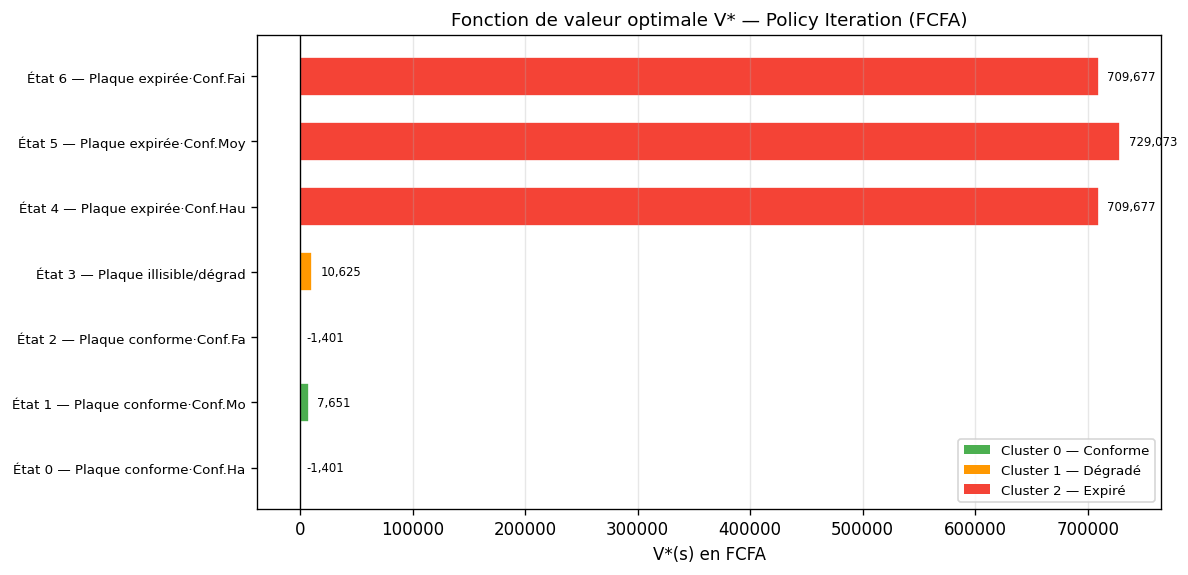
\includegraphics[width=0.85\textwidth]{figures/pi_value_function.png}
  \caption{Fonction de valeur $V^*(s)$ --- Policy Iteration ($\gamma=0.95$).
    Identique \`{a} celle obtenue par VI : valeurs \'{e}lev\'{e}es pour les
    \'{e}tats d'infractions fiscales (cluster~2, plaques expir\'{e}es).}
  \label{fig:pi_value_function}
\end{figure}}{}

\begin{table}[H]
\centering
\caption{Sensibilit\'{e} au facteur $\gamma$ --- Policy Iteration}
\label{tab:c:pi_sensitivity}
\begin{tabular}{rrrrr}
\toprule
$\gamma$ & It\'{e}r. globales & It\'{e}r. \'{e}val. cumul & Converg\'{e} & $\bar{V}^*$ (FCFA) \\
\midrule
  0.50 & 2 & 60 & Oui & 161\,591 \\
  0.70 & 2 & 116 & Oui & 164\,990 \\
  0.80 & 2 & 183 & Oui & 166\,781 \\
  0.90 & 3 & 576 & Oui & 176\,780 \\
  0.95 & 4 & 1735 & Oui & 309\,129 \\
  0.99 & 4 & 8832 & Oui & 1\,553\,100 \\

\bottomrule
\end{tabular}
\end{table}

\IfFileExists{figures/pi_gamma_sensitivity.png}{%
\begin{figure}[H]
  \centering
  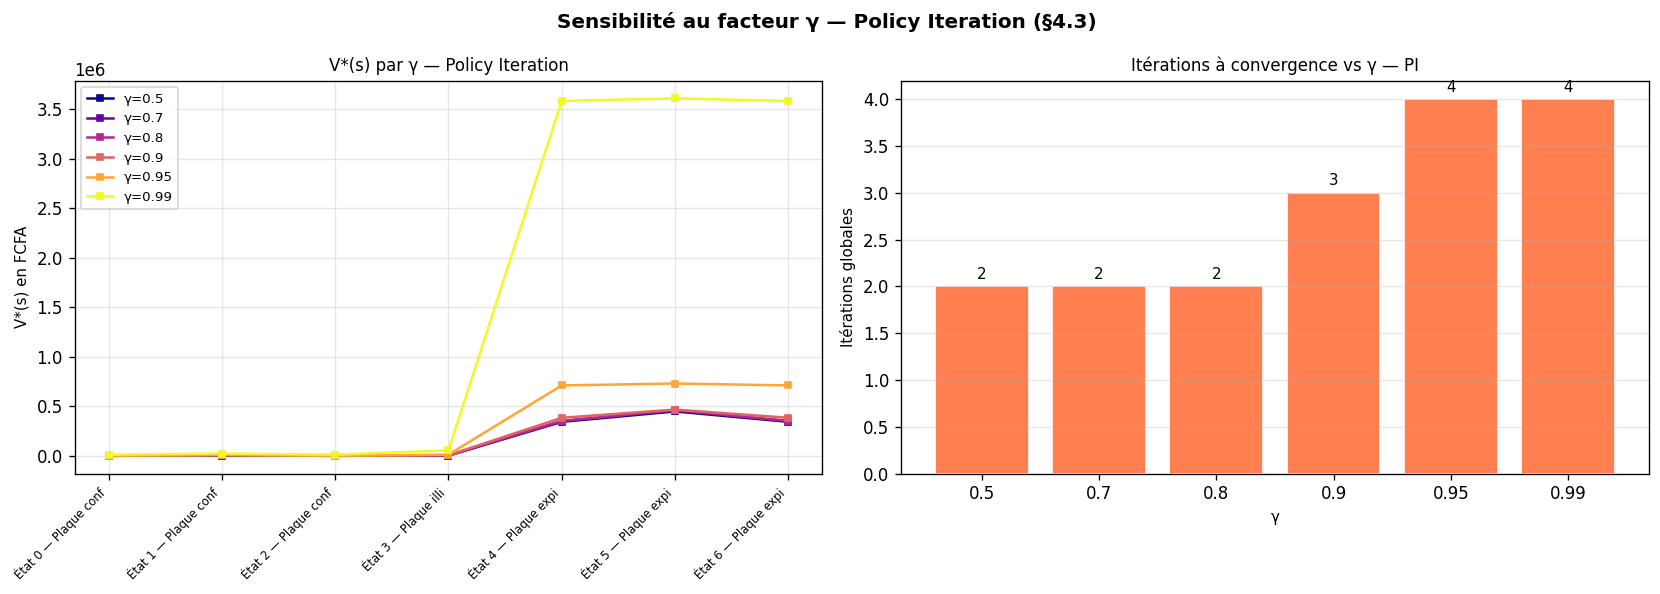
\includegraphics[width=0.85\textwidth]{figures/pi_gamma_sensitivity.png}
  \caption{Sensibilit\'{e} Policy Iteration au facteur $\gamma$ :
    it\'{e}rations globales et \'{e}valuations cumul\'{e}es.
    PI reste tr\`{e}s rapide ($\leq 4$ it\'{e}rations globales) quelle que soit
    la valeur de $\gamma$.}
  \label{fig:pi_gamma_sensitivity}
\end{figure}}{}

\paragraph{Interpr\'{e}tation m\'{e}tier MINT/DGI}
La politique $\pi^*$ obtenue par Policy Iteration confirm que les
plaques du cluster~2 (expir\'{e}es) doivent syst\'{e}matiquement faire
l'objet d'un \texttt{SIGNALEMENT\_DGI} quelle que soit la confiance OCR,
tandis que les plaques conformes \`{a} haute confiance sont laiss\'{e}es
passer. Cette politique est identique \`{a} celle de Value Iteration,
validant la robustesse du r\'{e}sultat.
L'avantage de PI est sa convergence rapide en quelques it\'{e}rations de
politique --- recommand\'{e}e pour une re-calibration p\'{e}riodique
du syst\`{e}me MINT/DGI avec de nouvelles donn\'{e}es de contr\^{o}le.